\textbf{Цель работы:} экспериментально исследовать свойства течения 
газов по тонким трубкам при различных числах Рейнольдса; выявить область 
применимости закона Пуазейля и с его помощью определить коэффициент вязкости воздуха.
\\\indent\textbf{Оборудование:} система подачи воздуха (компрессор, поводящие трубки); 
газовый счетчик барабанного типа; спиртовой микроманометр с регулируемым наклоном; 
набор трубок различного диаметра с выходами для подсоединения микроманометра; секундомер.

\section*{Теоретические сведения}
\indent Течение в трубе может быть либо ламинарным, либо турбулентным. 
При ламинарном течении слои жидкости не перемешиваются между собой.
Турбулентному течению характерны образование вихрей и активное перемешивание
слоев. Характер течения определяется числом Рейнольдса:
\begin{equation}
    Re = \frac{\rho u r}{\eta}
\end{equation}
С ростом числа Рейнольдса достигается его критическое значение($Re_{text{кр}} \approx 10^3$), при котором
характер течения из ламинарного переходит в турбулентное.
\indent Из закона Ньютона для силы вязкого трения в жидкостях и газах:
\begin{equation}
    \tau_{\text{xy}} = -\eta\frac{\partial v_{\text{x}}}{\partial y}
\end{equation}
следуют следующие формулы:
\begin{align}
    Q &= \frac{\pi R^4 \Delta P}{8 \eta l}\\
    u(r) &= \frac{\Delta P}{4 l}(R^2 - r^2)\\
    u_{\text{ср}} &= \frac{Q}{\pi R^2} = \frac{u_{\text{max}}}{2}
\end{align}

Ясно, что распределение скорости в трубе не будет пуазейлевским сразу. 
Оценим расстояние от начала трубы, на котором течение можно считать 
пуазейлевским:
\begin{align*}
    K &\sim \frac{1}{2}\rho u^2 \pi R^2 dx\\
    A_{\text{тр}} &\sim \eta\frac{du}{dr} 2\pi R dx l\\
    \frac{du}{dr} &\sim \frac{\Delta u}{R} \sim \frac{u}{R}\\
    Re &= \frac{K}{A_{\text{тр}}}\\
    l_{\text{пред}} &\sim R \cdot Re \\
\end{align*}
Примем $l_{\text{уст}} = 0.2R \cdot Re$\\\indent

\section*{Экспрериментальная установка}
\indent Поток воздуха поступает через газовый счетчик в трубку. Интенсивность подачи
воздуха регулируется краном. В разные части трубки можно подключать манометр,
чтобы измерять разность давлений на измеряемых концах трубки. С помощью
газового счетчика и секундомера измеряется средний объемный расход газа 
$Q = \frac{\Delta V}{\Delta t}$
\begin{figure}[h!]
    \centering
    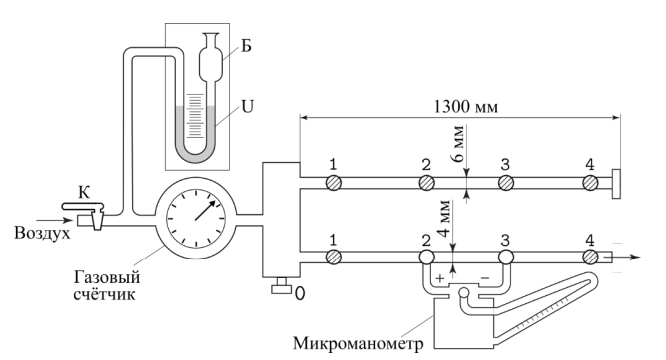
\includegraphics[width=12cm]{setup.png}
    \caption{Экспериментальная установка}
    \label{fig:setup}
\end{figure}

\section*{Экспрериментальные данные и ход работы}
Измерим параметры окружающей среды:
\begin{table}[h]
    \centering
    \begin{tabular}{|c|c|c|}
        \hline
        $P_{\text{атм}}$ , кПа& $\varphi$, \% & $t^\circ C$ \\\hline
         100.68 & 20 & 24.1\\\hline
    \end{tabular}
    \caption{Параметры окружающей среды}
\end{table}
\subsection*{Эксперимент на первой трубке}
$$d_{\text{труб}} = 3.95 \pm 0.05 \text{ мм}$$
$$l_{\text{труб}} = 90 \text{см}$$
\indent Расcчитаем значение $\Delta P_{\text{кр}}$ и $Q_{\text{кр}}$, при котором число Рейнольдса
станет равным критическому $Re{\text{кр}} \approx 10^3$. Для оценки 
будем считать $\eta \approx 2\cdot 10^{-5}$ Па$\cdot$с. Плотность воздуха из 
уравнения идеального газа:
\begin{equation}
    \rho = \frac{P \mu}{R T}
\end{equation}

% Here comes the talbe with outside data
\begin{table}[h!]
    \centering
    \begin{tabular}{|c|c|c|}
        \hline
        $\Delta P_{\text{кр}}$ , кПа/Дел& $Q_{\text{кр}}$, м$^3/$с $\cdot 10^{-5}$ & $l_{\text{кр}}$, см \\\hline
        182 / 92 & 10.8 & 39.5\\\hline
    \end{tabular}
    \caption{Критический объемный расход, давление и длина (k = 0.2)}
\end{table}

Определим $V_{\text{min}}$ и $t_{\text{min}}$, при которых относительная
погрешность измерения $Q$ не больше $\varepsilon = 1\%$.\\
$\sigma_{V} = 0.005$, тогда $V_{\text{min}} = \frac{\sigma_{\text{V}}}{\varepsilon} = 0.5$ л\\ 
Аналогично $t_{\text{min}} = \frac{\sigma_{\text{t}}}{\varepsilon}$, где
$$\sigma_{\text{t}} = \sqrt{\frac{\sum_{i=1}^{N} (t_{\text{ср}} - t_{\text{i}})^2}{N-1}} = 0.83\text{ с} \rightarrow t_{\text{min}} = 8.3\text{ с}$$
\begin{table}[h!]
    \centering
    \begin{tabular}{|c|c|c|c|c|c|c|c|}
        \hline
        №  & 1 & 2 & 3 & 4 & 5 & 6 & 7\\\hline 
        $t$ ,c& 5.97 & 5.77 & 5.88 & 5.76 & 5.74 & 5.72 & 5.84 \\\hline
    \end{tabular}
    \caption{Время прохождения $V_{\text{min}}$ объема газа}
\end{table}

\text{Теперь определим зависимость перепада давления от 
объемного расхода при ламинарном и турбулентном течении}
\begin{table}[h!]
    \centering
    \begin{tabular}{|c|c|c|c|c|c|c|c|}
        \hline
        №  & 1 & 2 & 3 & 4 & 5 & 6 & 7\\\hline 
        $t$ ,c& 38.47 & 26.85 & 20.23 & 16.92 & 13.25 & 11.62 & 10.87 \\\hline
        $\Delta P$, Дел & 20 & 30 & 40 & 50 & 60 & 71 & 80\\\hline 
        $Q$, мл & 11.36 & 17.61 & 24.17 & 38.82 & 48.92 & 61.12 & 71.43\\\hline 
    \end{tabular}
    \caption{Зависимость давления от объемного расхода $\Delta P(Q)$ 
    в ламинарном режиме\\ ($k = 0.2$)}
\end{table}

\begin{figure}[h!]
    \centering
    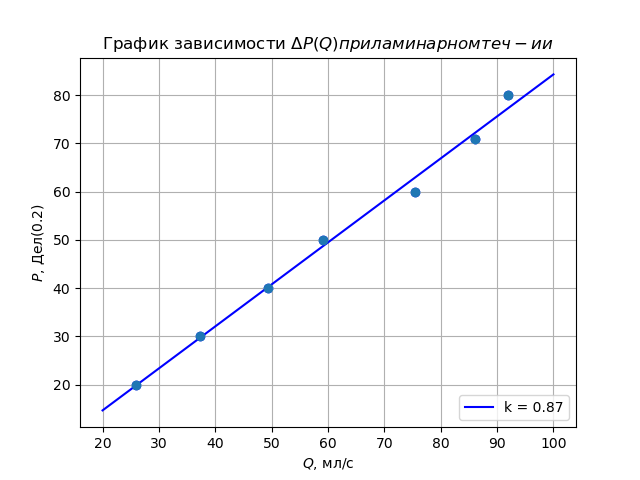
\includegraphics[width=12cm]{plot1.png}
    \caption{Зависимость давления от объемного расхода 
    при ламинарном течении}
    \label{fig:plot1}
\end{figure}

\text{В логарифмической шкале:}
\begin{figure}[h!]
    \centering
    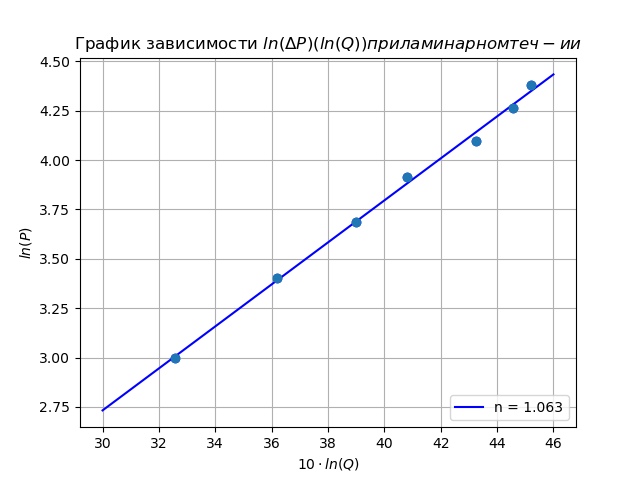
\includegraphics[width=12cm]{plot1ln.png}
    \caption{Логарифмическая ависимость давления от объемного расхода 
    при ламинарном течении}
    \label{fig:plot1ln}
\end{figure}

Итак из логирифмического графика видно, что при ламинарном течении
зависимость перепада давления от расхода линейная, что и было изложено 
в теории. Из первого графика, зная теперь угол наклона, можно определить 
значение коэффициента динамической вязкости воздуха $\eta$.
\begin{align}
    \eta = \frac{\pi R^4 \Delta P}{8 l Q} = 2.9 \cdot 10^{-5}
\end{align}

\begin{table}[h!]
    \centering
    \begin{tabular}{|c|c|c|c|c|c|c|c|}
        \hline
        №  & 1 & 2 & 3 & 4 & 5 & 6 & 7\\\hline 
        $\Delta P$, Дел & 80 & 100 & 120 & 140 & 160 & 180 & 200\\\hline 
        $Q$, мл & 90.17 & 97.47 & 104.82 & 108.54 & 114.59 & 124.9 & 126.58\\\hline 
    \end{tabular}
    \caption{Зависимость давления от объемного расхода $\Delta P(Q)$ 
    в турбулентном режиме\\ $(k = 0.4)$}
\end{table}

\begin{figure}[h!]
    \centering
    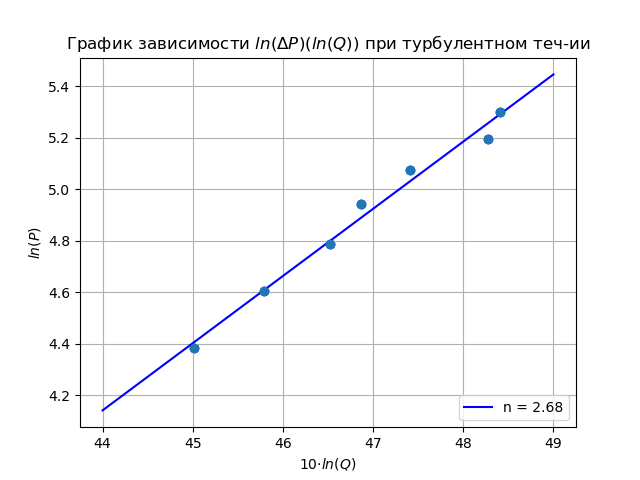
\includegraphics[width=12cm]{plot2.png}
    \caption{Зависимость давления от объемного расхода 
    при турбулентном течении}
    \label{fig:plot2}
\end{figure}
Здесь можно заметить, что степень зависимости находится между 2 и 3, тогда как в 
теоретических раскладках степень выходила равной 2. 

\begin{figure}[h!]
    \centering
    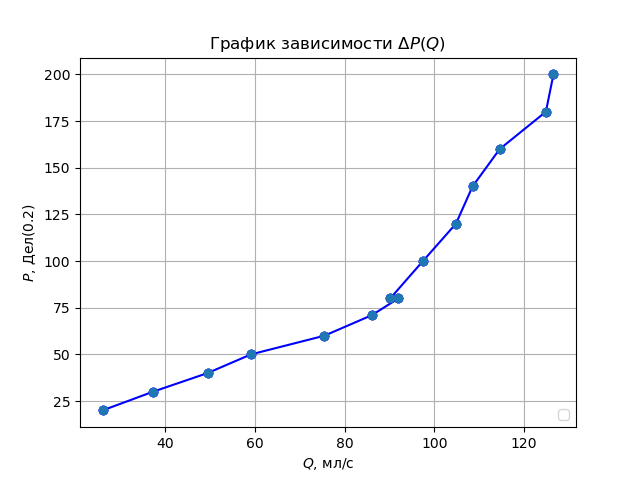
\includegraphics[width=12cm]{plotall1.png}
    \caption{Турбулентное и ламинарное течение}
    \label{fig:plotall1}
\end{figure}

По графику четко видно, что переход от ламинарного течения к турбулентному 
происходит при давлении в 80 Дел., в то время как в теории мы предположили
переход при $P_{\text{кр}} = 91$ Дел. 


\subsection*{Эксперимент на второй трубке}
$$d_{\text{труб}} = 5.3 \pm 0.05 \text{ мм}$$
$$l_{\text{труб}} = 90 \text{см}$$
\begin{table}[h]
    \centering
    \begin{tabular}{|c|c|c|}
        \hline
        $\Delta P_{\text{кр}}$ , кПа/Дел& $Q_{\text{кр}}$, м$^3/$с $\cdot 10^{-5}$ & $l_{\text{кр}}$, см \\\hline
        135 / 68 & 14 & 53\\\hline
    \end{tabular}
    \caption{Критический объемный расход, давление и длина (k = 0.2)}
\end{table}


\text{Определим зависимость перепада давления от 
объемного расхода при ламинарном и турбулентном течении}
\begin{table}[h!]
    \centering
    \begin{tabular}{|c|c|c|c|c|c|c|c|}
        \hline
        №  & 1 & 2 & 3 & 4 & 5 & 6 & 7\\\hline 
        $\Delta P$, Дел & 10 & 15 & 20 & 25 & 30 & 35 & 40\\\hline 
        $Q$, мл & 28.04 & 43.98 & 55.68 & 76.57 & 89.45 & 102.15 & 117.23\\\hline 
    \end{tabular}
    \caption{Зависимость давления от объемного расхода $\Delta P(Q)$ 
    в ламинарном режиме\\ ($k = 0.2$)}
\end{table}

\begin{figure}[h!]
    \centering
    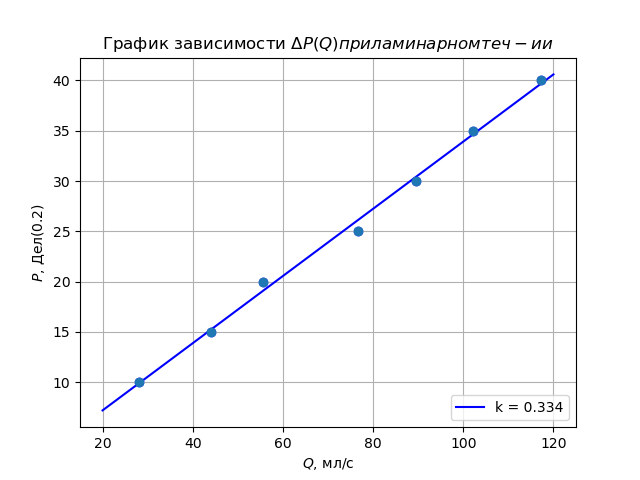
\includegraphics[width=12cm]{plot3.png}
    \caption{Зависимость давления от объемного расхода 
    при ламинарном течении}
    \label{fig:plot3}
\end{figure}

\text{В логарифмической шкале:}
\begin{figure}[h!]
    \centering
    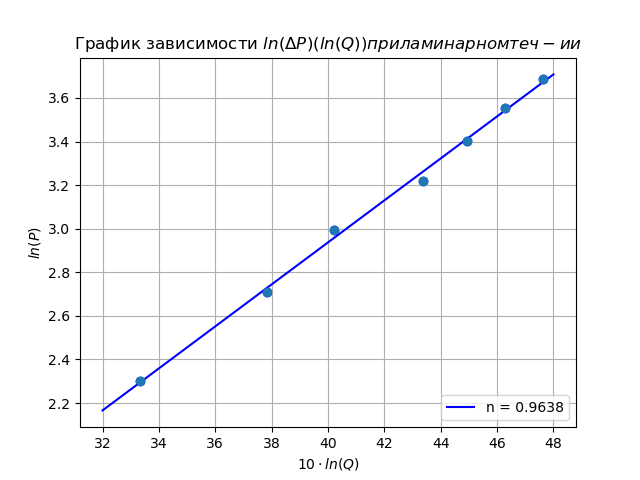
\includegraphics[width=12cm]{plot3ln.png}
    \caption{Логарифмическая ависимость давления от объемного расхода 
    при ламинарном течении}
    \label{fig:plot3ln}
\end{figure}

Итак из логирифмического графика видно, что при ламинарном течении
зависимость перепада давления от расхода линейная, что и было изложено 
в теории. Из первого графика, зная теперь угол наклона, можно определить 
значение коэффициента динамической вязкости воздуха $\eta$.
\begin{align}
    \eta = \frac{\pi R^4 \Delta P}{8 l Q} = 2.7 \cdot 10^{-5} \text{ Па$\cdot$с}
\end{align}

\begin{table}[h!]
    \centering
    \begin{tabular}{|c|c|c|c|c|c|c|c|}
        \hline
        №  & 1 & 2 & 3 & 4 & 5 & 6 & 7\\\hline 
        $\Delta P$, Дел & 70 & 90 & 100 & 110 & 120 & 130 & 140\\\hline 
        $Q$, мл & 196.08 & 203.67 & 220.91 & 224.22 & 231.66 & 241.16 & 251.47\\\hline 
    \end{tabular}
    \caption{Зависимость давления от объемного расхода $\Delta P(Q)$ 
    в турбулентном режиме\\ $(k = 0.2)$}
\end{table}

\begin{figure}[h!]
    \centering
    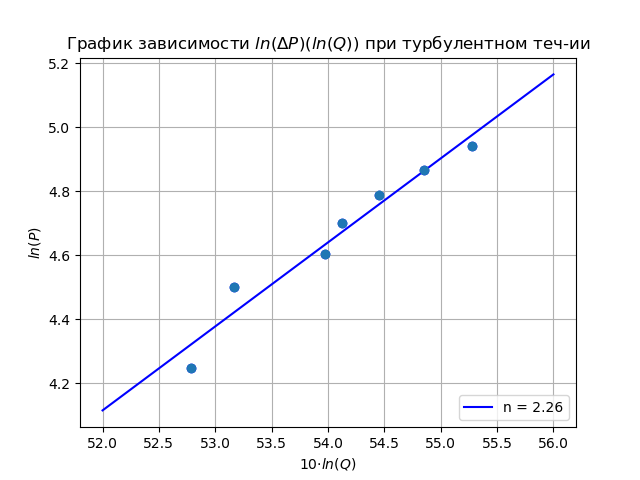
\includegraphics[width=12cm]{plot4.png}
    \caption{Зависимость давления от объемного расхода 
    при турбулентном течении}
    \label{fig:plot4}
\end{figure}
Здесь можно заметить, что степень зависимости находится между 2 и 3, тогда как в 
теоретических раскладках степень выходила равной 2. 

\begin{figure}[h!]
    \centering
    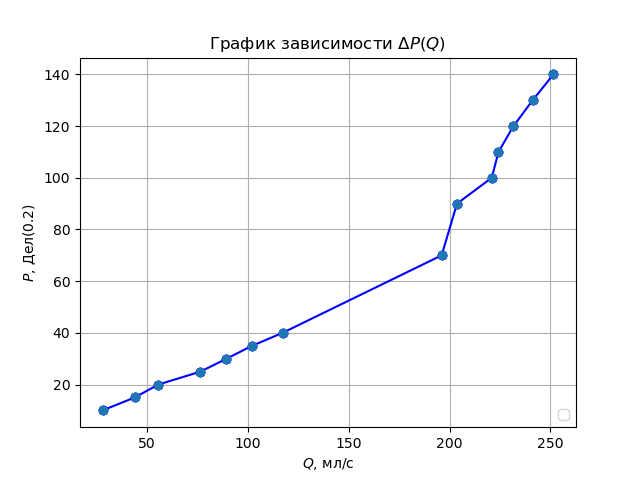
\includegraphics[width=12cm]{plotall2.png}
    \caption{Турбулентное и ламинарное течение}
    \label{fig:plotall2}
\end{figure}

По графику четко видно, что переход от ламинарного течения к турбулентному 
происходит при давлении в 70 Дел., в то время как в теории мы предположили
переход при $P_{\text{кр}} = 68$ Дел. 

\section*{Результаты и выводы}
Погрешность вычисления коэффициента динамической вязкости можно оценить как
$\varepsilon_{\eta} = \sqrt{1 + 1 + (4*1)^2} \approx 4.2 \%$
(1\% погрешность определения $Q$, 1\% погрешность определения длины трубки, и 16\% 
от радиуса трубки т.к он входит со степенью 4)\\
\indent \textbf{1)Определение границы перехода от ламинарного течения к турбулентному:}\\ 
Из графика можно определить границу перехода, т.к резко меняется наклон. Соответственно
посчитаем критическое значение числа Рейнольдса для двух трубок:\\ 
$$Re_{\text{кр}} = \frac{\rho Q_{\text{кр}}}{\pi R \eta}$$
$Re_1 \approx 570$;   $Re_2$ \approx 995 \approx $10^3$\\ 
Как видим число Рейнольдса почти совпадает с предполагаемым равным $10^3$.\\ 
\textbf{2)Зависимость перепада давлений от объемного расхода при ламинарном течении:}\\ 
Эта зависимость действительно оказалась линейной, как и предполагалось в теории. Из
этого так же следует, что критическая длина трубки была так же определена верна и к
моменту измерения распределение скоростей было пуассоновским. \\
\textbf{3)Определение коэф. динамической вязкости:}\\ 
С помощью графика зависимости давления от расхода было найдено значение динамической вязкости
при ламинарном течении. Оно оказалось чуть больше, чем было предположено
(2.7 > 2). 
